Основой современного ассистента является большая языкова модель. Термин большая на текущий момент
означает число параметров модель большее одного миллиарда. Таким образом, физическая запись модель требует
значительно ресурса памяти большое нескольких гигабайт, что и послужило причиной названия.  

Обучение языковых моделей для задач ассистирования разделяется на два этапа предобучение (\textit{англ.} pretrain) и инструкционное дообучение.
В ходе первого этапа модель обучается синтаксической структуре языка. 
Во втором обучается под руководством эксперта на специализированных корпусах инструкций. Таковыми, например, могут являться
дача структурированных определений, изложение информации в специальной стилистической форме, поиск ключевых слов в массивном тексте.

\begin{figure}[h]
    \centering
    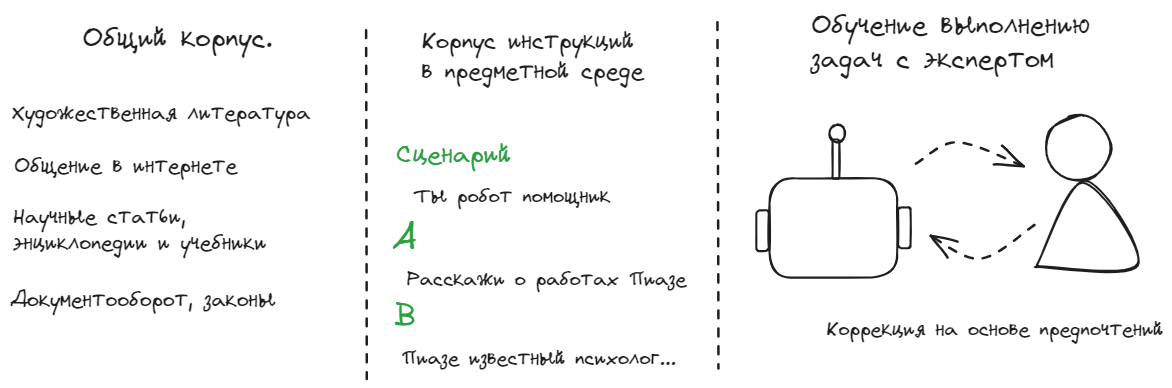
\includegraphics[width=0.5\textwidth]{assets/work/arch/learning.excalidraw.png}
    \caption{Обучение разбито на три ключевых этапа: подготовка, адаптация на корпусе}
    \label{train}
\end{figure}


Предобучение требует значительных вычислительных ресурсов, 
не всегда доступных в образовательных и научных
целях. В связи с этим компании, обладающие достаточным
ресурсом выкладывают свои модели в общий доступ \cite{jiang2023mistral}\cite{jiang2024mixtral}\cite{touvron2023llama}


Для оценки способностей языковых моделей создаются специальные системы тестирования количественно оценивающие способности моделей к \begin{itemize}
    \item способности к пересказу
    \item умение переводить
    \item понимание животного и растительного мера 
    \item решение аналитических задач 
\end{itemize}


\begin{figure}[h]
    \centering
    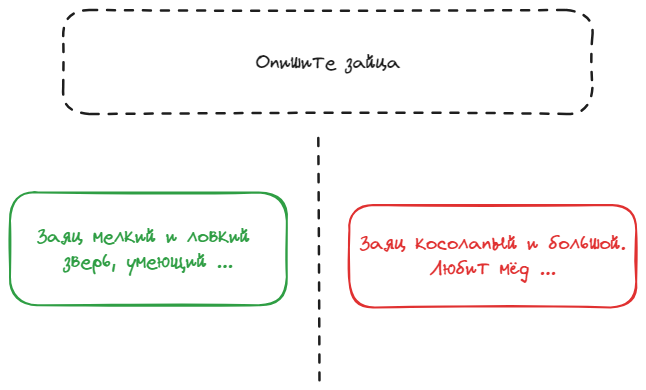
\includegraphics[width=0.5\textwidth]{assets/work/arch/instruction.excalidraw.png}
    \caption{Адаптация выполнять задачи проходит через взаимодействие с пользователем и работу эксперта}
    \label{instruction}
\end{figure}

Для сравнения моделей также используется техника попарного сравнения модели. 
Таким образом, исходя из предпочтений пользователей, выносится оценка модели.

Большие языковые модели не гарантируют корректное исполнение даже базовых арифметических операций сложения . 
В обзоре \cite{zhao2023survey} показано, что подобные проблемы возникают во многих строгих постановках, где
соблюдение формы требует интеллектуального участия \begin{itemize}
    \item написание исполняемого языком программирования кода
    \item переход в математических выражениях.
\end{itemize} 

Для разрешения проблемы исследователи предложили использование инструментов,
которые используются моделью для качественного выполнения инструкции. На данный момент сложились \begin{itemize}
    \item обращения к информационным системам  (RAG - retreival augmented generation)\cite{lewis2020retrieval}
    \item работа с средой исполнения программного кода \cite{parisi2022talm}
    \item генерация сопровождающей иллюстрации
\end{itemize}

К текущему моменту 

Для оценки способностей языковых моделей создаются специальные системы тестирования количественно оценивающие способности моделей к \begin{itemize}
    \item способности к пересказу
    \item умение переводить
    \item понимание животного и растительного мера 
    \item решение аналитических задач 
\end{itemize}








